\section{The sample}
\label{sec:sample}

This search covers \NWindows{} spectral windows toward \NStars{} stars in
\NSystems{} systems within 40\,pc, where a \emph{system} is a bound group,
counted once however many of its stars were observed. The windows come from
\NEB{} public ALMA execution blocks, all put through the same pipeline:
\TotalDataTB\,TB of raw data, \StTelHours\,h of telescope time and
\LdgCensusHours\,h summed over windows. We call this set the \emph{primary
census}. Every expectation in the paper, and every limit of
\S\ref{sec:pninetysel} and Table~\ref{tab:persys}, is computed over it and
nothing else. It holds \CsNCross{} threshold crossings
(Table~\ref{tab:blockledger}b, row~\CtRowCensusCross), all in quality-passing data, one of them toward
\CtUncatStar, which lies in a census window but has no catalogue row.
That crossing is \MbUncatAttrWord{} (\MbUncatTrans{} at \MbUncatDv\,km\,s$^{-1}$
in the star's frame). Because its own position has no catalogue row, it
stands on neither side of the chance comparison, and its window enters the
expectation once, through the control positions around \MbUncatHost{}
(Appendix~\ref{app:falsealarm}).

Some data were searched after the census was closed, and these are kept
apart. A further \CeNTailCross{} crossings lie in an \emph{archival tail} of
\LdgExtTail{} blocks toward \LdgTailStars{} census stars, and they enter no
expectation. Nor do an archival extension, a reserved \emph{hold-out}
(Appendix~\ref{sec:heldout}) and a control beyond 40\,pc
(\S\ref{sec:holdoutsearch}). Table~\ref{tab:blockledger} accounts for every
block in every set.

The census divides into two experiments by native channel width, since both
the search statistic and the completeness calibration depend on it.
\emph{Class~A}, the primary experiment, is the \NWinA{} fine-channel windows
toward \LdgClassAStars{} stars in \NSysClassA{} systems. Of these,
\EtaDriftAOk{} are channelised finely enough for the searched drift to cross a
channel (\S\ref{sec:statistic}), and every sensitivity and limit quoted is
Class~A's unless stated otherwise. \emph{Class~B}, the other \NWinB{}
windows, supports a secondary search for an unresolved narrowband spectral
excess. The channelisation of these windows is bimodal, so the division is
unambiguous: the widest fine channel is \ScChanFineMaxMHz\,MHz and the
narrowest coarse one \ScChanCoarseMinMHz\,MHz, with nothing in between.

A star enters the sample if its Gaia~DR3 parallax is at least 25\,mas and
measured to better than \PlxAdqlPct{} per cent, and if it is brighter than
$G=\SfCensusGLim$. In practice the precision condition
never binds, since the least precise parallax among the stars
searched has an uncertainty of \SfPlxWorstPct{} per cent.
Its proper-motion-corrected position must also fall inside the quoted field
of view of a public execution block, though not necessarily at the pointing
centre, and its distance is taken as $1/\varpi$. A window is kept only where
the primary-beam response at the star is at least \BmFloorResp. At that level
the adopted Gaussian beam and a blocked-aperture response part by
\BmFloorTolPct{} per cent, and no window falls below it
(Appendix~\ref{app:pbresp}). One serendipitous field star is named throughout
after the ALMA source at the centre of its field, \BkAlmaName. It is
\BkAlmaTwoMass{} (Gaia~DR3 \BkAlmaGaia), an \BkAlmaSpType{} dwarf at
\BkAlmaDistPc\,pc with no catalogued radial velocity.

The Gaia requirement has a cost at the bright end, since a star with no
Gaia~DR3 parallax cannot enter the sample. It removes all \BsNBright{} stars
in this volume brighter than \BsBrightMag{} magnitude, and \BsNGap{} of its
\BsNVol{} Hipparcos stars. Of these, \BsNAlmaWord{} (\BsStarList) lie in
public fields, with \BsNWinA{} fine-channel and \BsNWinB{} coarse-channel
windows that a search admitting Hipparcos astrometry could add.


\subsection{The archival selection}
\label{sec:bias}

This sample was not designed. It is whatever ALMA programmes with other aims
happened to observe among the stars Gaia~DR3 catalogues, and
\PctDiscProposal{} per cent of the stars searched were targeted under a
debris-disc or planet-formation proposal. Table~\ref{tab:selfunc} measures the
resulting bias against the Gaia~DR3 census of which the searched stars are a
subset ($\varpi>0$, $\sigma_\varpi/\varpi\le\SfPlxCutDec$,
$1/\varpi\le40$\,pc, $G<\SfCensusGLim$; \SfCensusN{} objects). That census
is limited in magnitude as well as in volume. Both columns of the table come
from the same extract and are classified by BP$-$RP colour, with absolute $G$ magnitude separating the degenerates.

Distance is the dominant selection effect. Stars within 5\,pc are
over-represented by a factor \SfTopRatio, and the excess declines
monotonically to a factor of two \emph{under}-representation beyond 30\,pc. Colour comes
second. A~stars are over-represented by a factor of about \SfARatio{} and F and G stars
by factors of three, because those are the stars with bright debris discs.
For the A~stars that factor is a floor, since the Gaia requirement
itself removes stars as blue as these at \BsEarlyRatio{} times its rate among
the others. M~dwarfs, on the other hand, are depleted. They make up
\SfMSearched{} of the \SfNMain{} non-degenerate stars among the \SfNStar{}
searched, a factor \SfMRatio{} of their share of the census, and only
\SfMClassAStars{} of them carry fine-channel coverage. Coverage is also concentrated, with
\ConcThreeWin{} of the \NWindows{} windows coming from \ConcThreeSys{}
systems.

The selection acts hardest on the targets a designed search would pick. Of
the \CsIntNRow{} sample systems within 15\,pc with a confirmed planet,
\CsIntNoClassA{} have no Class~A coverage and so no drift-resolving limit.
No statement in this paper is therefore an occurrence rate for the solar
neighbourhood.

%% GENERATED by selfunc_v411.py -- do not hand-edit.
\begin{table}
\centering
\scriptsize
\setlength{\tabcolsep}{4pt}
\caption{Selection function of the 90 searched stars against the Gaia~DR3 census of \S\ref{sec:bias} (within 40\,pc, $G<16$). ``Ratio'': the searched over the census column fraction.}
\label{tab:selfunc}
\begin{tabular}{@{}lrrr@{}}
\toprule
Property & Census & Searched & Ratio \\
\midrule
\multicolumn{4}{@{}l}{Distance} \\
\quad $d\le5$\,pc & 48 (0.3\%) & 13 (14.4\%) & 52.9 \\
\quad 5--10\,pc & 240 (1.4\%) & 13 (14.4\%) & 10.6 \\
\quad 10--20\,pc & 2069 (11.8\%) & 18 (20.0\%) & 1.7 \\
\quad 20--30\,pc & 5391 (30.7\%) & 19 (21.1\%) & 0.7 \\
\quad 30--40\,pc & 9818 (55.9\%) & 27 (30.0\%) & 0.5 \\
\midrule
\multicolumn{4}{@{}l}{Colour class$^{a}$} \\
\quad A & 61 (0.4\%) & 5 (6.2\%) & 17.2 \\
\quad F & 473 (2.8\%) & 8 (10.0\%) & 3.6 \\
\quad G & 978 (5.8\%) & 15 (18.8\%) & 3.2 \\
\quad K & 2221 (13.2\%) & 11 (13.8\%) & 1.0 \\
\quad M & 13\,082 (77.8\%) & 41 (51.2\%) & 0.7 \\
\midrule
\multicolumn{4}{@{}l}{Other axes} \\
\quad Confirmed planet hosts$^{b}$ & 26 (15.5\%) & 24 (26.7\%) & 1.7 \\
\quad White dwarfs$^{a}$ & 463 (2.7\%) & 8 (9.1\%) & 3.4 \\
\quad Searched stars / systems & -- & 90 / 83 & -- \\
\bottomrule
\end{tabular}

\smallskip
{\footnotesize $^{a}$Colour bins, not MK types: BP$-$RP $<0.36$ for A, 0.36--0.72 for F, 0.72--0.95 for G, 0.95--1.77 for K and $>1.77$ for M, where the census's own temperature--colour relation crosses 7500, 6000, 5300 and 3900\,K. Degenerate: more than 4\,mag below the census main sequence. The five classes are normalised over the 80 non-degenerate searched stars and the 16\,815 non-degenerate census objects, the degenerate row over the 88 classified searched stars and the 17\,278 classified census objects.\\ $^{b}$Both columns are the same positional join, of the 168-entry ALMA-covered work list and of its searched subset, to the NASA Exoplanet Archive \texttt{pscomppars} table accessed 2026 October 4. The 24 searched hosts carry 51 confirmed planets, 22 of the 24 surviving the deuterium-burning mass limit; the Gaia census carries no planet information, so the census column in this row is the work list and not the 17\,566-object Gaia census.}
\end{table}


\subsection{Frequency coverage and archival scope}
\label{sec:coverage}

The Class~A experiment covers $\Delta\nu_A=\DnuA$\,GHz of unique sky
frequency, in \DomAIslands{} disjoint islands between \DomAFreqLo{} and
\DomAFreqHi\,GHz rather than a continuous band. With the coarse-channel
windows the coverage is \DnuAB\,GHz in \UnionIntervals{} intervals, of which
\SearchedUnionGHz\,GHz survives the molecular-line mask of
\S\ref{sec:summary}. Fig.~\ref{fig:waterfall} shows how that coverage is
distributed. A transmitter between the islands was never observable here,
whatever its power. Nor is the archive exhausted: \LdgExtScope{} further
blocks inside the same query were unprocessed when the census was frozen,
\FateNoCal{} of them because the archive holds their raw visibilities but
never pipeline-calibrated them (Table~\ref{tab:blockledger}).

\begin{figure*}
\centering
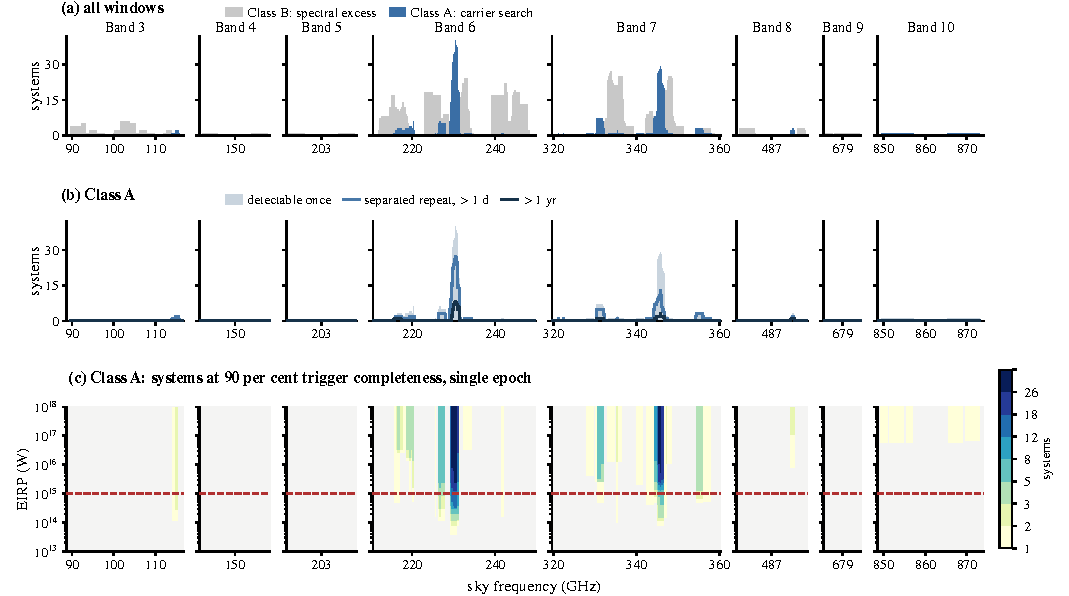
\includegraphics[width=\textwidth]{figures/coverage_r27.pdf}
\caption{\textbf{Where this survey searched, and where a repeat could test
it}: independent systems covering each sky frequency, one panel per populated
ALMA band, its width proportional to the band's frequency share; curves step
at the searched window edges. \emph{(a)}~Every window: blue, the
fine-channel carrier search (Class~A); grey, the coarse-channel
spectral-excess search (Class~B); the summed window bandwidth is
$\GrossOverUnion\times$ the union. \emph{(b)}~Class~A: detectable once (grey);
with a \emph{separated} block (\S\ref{sec:summary}) covering the
frequency (blue); beyond a year (dark). An accelerating carrier further needs
a predicted frequency within the repeat coverage, with adequate sensitivity.
\emph{(c)}~Class~A systems in which a carrier of that EIRP reaches the
threshold nine times in ten in one epoch; dashed, $\CovEirpRefTex$\,W.}
\label{fig:waterfall}
\end{figure*}
